\documentclass[11pt,a4paper]{article}
\usepackage{alltt}
\usepackage{tikz}
\usepackage{amsthm}
\usetikzlibrary{arrows}
\usetikzlibrary{automata,positioning}
\newcommand*{\DashedArrow}[1][]{\mathbin{\tikz [baseline=-0.25ex,-latex, dashed,#1] \draw [#1] (0pt,0.5ex) -- (1.3em,0.5ex);}}%
\begin{document}
\title{\huge Wijsbegeerte}
\author{Ward Schodts}
\date{}
\maketitle


\section*{\centering \underline{Deel 1: Interesses, instrumenteel en intrinsiek}}

\section{De ervaringsmachine}
\subsection{De droommachine}
\newtheorem*{-R}{Principe -R - Alles is ervaring}
\begin{-R}
De dingen hebben geen belang, tenzij door hun waarde voor ons.
\end{-R}
\newtheorem*{+R}{Principe +R - Ervaring is niet alles}
\begin{+R}
De dingen hebben geen belang, tenzij door hun waarde voor ons.
\end{+R}
\begin{itemize}
\item Solipsisme: de filosofie dat er maar een enkel bewustzijn bestaat: dat van de waarnemer.
\end{itemize}
\begin{tabular}{p{7cm} p{6cm}}
	\hline
	
	 \raggedright Mephisto & Maniphesta\\
	\hline
	\begin{flushleft}
	\begin{enumerate}
	
	\item[Arg. 1:] nieuwsgierigheid
	\item[Arg. 2:] geen negatieve bijwerkingen, \\geen kater
	\item[Arg. 3:] unieke ervaring
	\item[Arg. 4:] ultieme genieting
	\item[Arg. 5:] antwoord: onechte ervaring \\bestaat niet
	\end{enumerate}	 
	\end{flushleft}
	
	&
	\begin{flushleft}
	
	\begin{enumerate}
	\item[Tegenarg. 1:] vereiste van onvoorspelbaarheid
	\item[Tegenarg. 2:] onbelsist, prijs=solipsisme
	\item[Tegenarg. 3:] o.k. maar te makkelijk, geen verdienste
	\item[Tegenarg. 4:] neutraal, voorspelbaar, verveling
	\item[Tegenarg. 5:] aan: zelfbedrog!
	\item[Tegenarg. 6:] weerlegging: echte ervaring $\neq$ ervaring van het echte!
	\end{enumerate}
	\end{flushleft}


	\\
	
	\hline
	
\end{tabular}
\\
\\
Paradox:
\begin{itemize}
\item We zijn gericht op het ervaarbare
\item Anderzijds blijken we gericht te zijn op het niet-ervaarbare
\end{itemize}
\subsection{Alles is ervaringsmachine}
Zodra we beseffen dat het om een ervaringsmachine gaat, een soort verslaving, zijn we niet trots er aan te liggen. 
Beheersingsinteresse of interesse in controle. 
Al bezig met onze eigen ervaringsmachine rondom ons te bouwen, we zitten er al middenin.
\\
SAINT-EXUPERY
\\
\\
Herformulering van de paradox hierboven:
\begin{itemize}
\item We verlang het beheersbare = wat aan ons verlangen beantwoordt. 
\item We verlangen het onbeheersbare = wat niet aan ons verlangen beantwoordt!
\end{itemize}


\section{Alles is beheersing}
Eerste hypothese over de menselijke interesses: alle interesse is uiteindelijk beheersingsinteresse.

\subsection{Alles is techniek}
Praktische beheersing van de wereld neemt twee vormen aan:
\begin{itemize}
\item Technische maakbaarheid
\item Overlevingswaarde
\end{itemize}
Technische interesse: het maken en hermaken van de wereld is wat ons bezighoudt, ook indien niet alles effectief maakbaar zou blijken.
\subsubsection*{Machineconcepten}
Machinerevolutie doorheen de geschiedenis:
\begin{itemize}
\item Handenarbeid werd omgezet in energie of beweging.
\item Werden verder uitgewerkt totdat alle enerie in elkaar kon getransformeerd worden.
\item Ontstaan cognitieve kennismachine: computer.
\end{itemize}
Kan een machine denken of is wat wij doen, als we denken een machinaal gebeuren?\\ 
Kwestie van \textit{mind en brain} gaat voortaan over de driehoek tussen het biologische het psychische \'en het machinale.
\subsubsection*{Het paradijs van de techniek}
Technische utopie $\rightarrow$ d\'e weg van de verbetering is de eg van de techniek. Voor elk oplosbaar probleem is de oplossing een technische oplossing. Gaat zelfs zo ver tot onze eigen maakbaarheid...
\subsubsection*{De paradox van de techniek}
We worden beheerst door het instrument dat we uitvonden om de natuur te beheersen, \'en door onze beheersingsdrift zelf, die onbeheersbaar is geworden, een misplaatste fascinatie.
\\
Martin HEIDEGGER (1889-1976): "voor elke technische oplossing duikt een nieuw (en groter) probleem op."
\subsection{Alles is selectie}
Onze interesses liggen in het verlengde van de overleving. We zijn overlevingsmachines.
\\
De tweede versie van de eerste hypothese: alles wat ons zou kunnen interesseren buiten de overleving is ofwel een onrechtstreekse bijdrage tot de overleving, ofwel een uitbreiding ervan: het verbeteren van onze levenscondities zoals in de "alles is techniek"-versie.
\\
$\rightarrow$ ingebakken in de common sense over leven
\\
\\
ARISTOTELES geloofde niet in een schepping van de wereld, maar in eeuwig bestaan en aan zichzelf gelijkblijvende soorten. (Deze visie was er ook tijdens de middeleeuwen)
\\
NEWTON: de ontstaanswetten, ontwikkelingswetten zijn niet te achterhalen omdat ze niet bestonden. Vragen achter evolutie lag in het terrein van het metafysische en theologische.
Tijdgenoten en voorlopers van DARWIN die haar aan twijfelden:
\begin{itemize}
\item Buffon
\item Maupertuis
\item Goethe
\item Lyell
\item Lamarck
\item Paley
\end{itemize}
DARWIN: het gaan niet allleeen om een blinde drang om in zijn bestaan te volharden. De hele ontwikkeling van de levende soorten is geleid door overlevingswaarden. \\Hij had als eerste een verklaring: evolutie van de soorten.
\\
\begin{center}
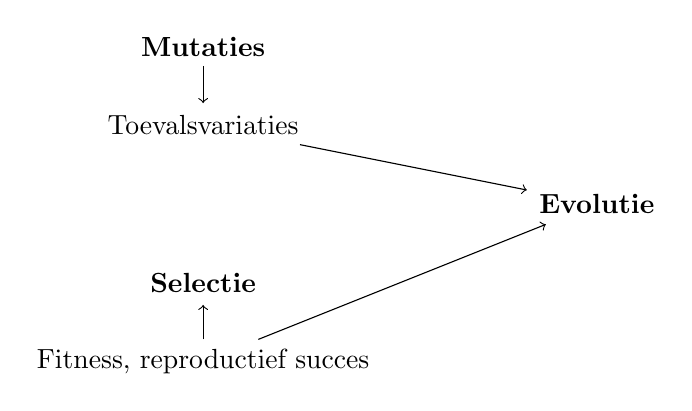
\begin{tikzpicture}[shorten >=1pt,node distance=2cm,on grid,auto] 
\node (a) at (0,-10) {\textbf{Mutaties}};
\node (b) at (0,-11) {Toevalsvariaties};
\node (c) at (5,-12) {\textbf{Evolutie}};
\node (d) at (0,-13) {\textbf{Selectie}};
\node (e) at (0,-14) {Fitness, reproductief succes};

\path
(a) edge[->] (b)
(e) edge[->] (d)
(b) edge[->] (c)
(e) edge[->] (c);
\end{tikzpicture}
\end{center}
Naast adaptaties zeggen GOULD en LEWONTIN:
\\
\textbf{exaptatie:} onvoorziene neveneffecten van veranderingen zoals:
\begin{itemize}
\item Vleugels van vogels
\item Duim van de panda
\end{itemize}
\textbf{Sociobiologie:} (nu \textit{evolutionaire psychologie}) is een versie van het neodarwinisme waarbij men een volledige verklaring van de cultuur en de menselijke ervaring in het verlengde van de darwinistische categorie\"en van overleving, selectie, mutatie, variatie en reproductief succes op het oog heeft.
\\
\\
DAWKINS, RUSE en WILSON:
\\
Psychologische en culturele eigenschappen moeten net als strikt biologische trekken verklaard worden vanuit het evolutionair voordeel dat zij opleveren. Zoals co\"operatie.
\\
Net zoals genen in de natuur eenheden van reproductie zijn zijn in de cultuur ook dergelijke eenheden (memen) (gedragingen edl) die zich door imitatie doorzetten . Omvorming in de loop van dat proces is dan niet het resultaat van culturele evolutie dan wel de selectie van de meest succesvolle kopieerbare items.

\subsection{Morele intu\"ities}
E.O. WILSON: alle hooggestemde waarden zijn overlevingswaarden in vermomming.
Er zijn 2 problemen mbt de sociobiologische opvatting van cultuur:
\begin{enumerate}
\item[1.] \underline{Het etische of morele:}
\\
Welk is de ware aard van onze morele principes volgens de sociobiologen?
Al onze morele waarden zijn eigenlijk overlevingswaarden in vermomming, kan ook indirect:
\begin{itemize}
\item[bv.] We kunnen in pure cultuur en kunst geïnteresseerd zijn maar dat is maar omwille van de complexe noden en verlangens die onze maatschappij en haar diverse groepen vertonen : deze zijn voor hun collectieve overleving afhankelijk van tal van niet-direct nuttige activiteiten die de samenhang en neiging tot coöperatie bevorderen.
\item[bv.] Altruïsme is niets anders dan eigenbelang
Maar zijn dit dan nog morele waarden? De eis andere mensen te respecteren als personen kan niet berusten op het feit dat ze ons nog van pas kunnen komen.
\end{itemize}

\end{enumerate}

\subsection{Taal: Venus van de sterren, emergente symbolen}
\begin{enumerate}
\item[2] \underline{Taal:}
\\
Introductie van taal: exponenti\"ele versnelling in de culutuur? Is taal de sprong van natuur naar cultuur - of een voortzetting van mutaties en selecties?
\\
Voor de sociobiologen is de mensentaal een simpel verlengstuk van de tekentaal van de dieren.
\\
$\leftrightarrow$ Voor de tegenstanders is taal per definitie mensentaal en een radicaal nieuw verschijnsel in de natuur.
\\
\\
Susanne LANGER:
Taal is continu opgestegen uit de signaalsystemen van de hogere diersoorten maar is tevens discontinu daarmee in de zin dat het gaat om de emergentie van iets met nieuwe eigenschappen.

\begin{center}
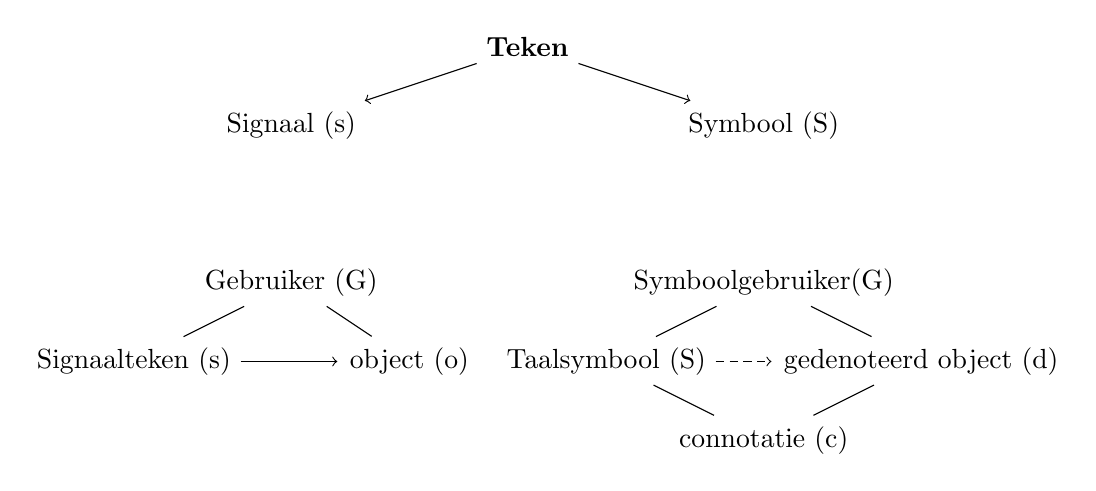
\begin{tikzpicture}[shorten >=1pt,node distance=2cm,on grid,auto] 
\node (a) at (3,0) {\textbf{Teken}};
\node (b) at (0,-1) {Signaal (s)};
\node (c) at (6,-1) {Symbool (S)};
\node (d) at (0,-3) {Gebruiker (G)};
\node (e) at (6,-3) {Symboolgebruiker(G)};
\node (f) at (-2,-4) {Signaalteken (s)};
\node (g) at (1.5,-4) {object (o)};
\node (h) at (4,-4) {Taalsymbool (S)};
\node (i) at (6,-4) {};
\node (j) at (8,-4) {gedenoteerd object (d)};
\node (k) at (6,-5) {connotatie (c)};

\path
(a) edge[->] (b)
(a) edge[->] (c)
(d) edge[-] (f)
(d) edge[-] (g)
(f) edge[->] (g)
(e) edge[-] (h)
(e) edge[-] (j)
(h) edge[-] (k)
(h) edge[->,densely dashed] (j)
(j) edge[-] (k);
\end{tikzpicture}
\end{center}
$\DashedArrow[->,densely dashed    ]$ steeds omweg over mentale conceptatie om tot "d" te komen.
\\

\textbf{Connotatie:} inhoud van het begrip of intensie.
\\
\textbf{Denotatie:} omvang van het gezegde of extensie.
\\
\begin{center}
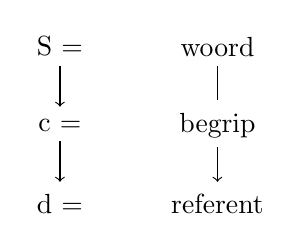
\begin{tikzpicture}[shorten >=1pt,node distance=2cm,on grid,auto] 
\node (a) at (0,0) {S   =};
\node (b) at (2,0) {woord};
\node (c) at (0,-1) {c =  };
\node (d) at (2,-1) {begrip};
\node (e) at (0,-2) {d =};
\node (f) at (2,-2) {referent};


\path

(a) edge[->] (c)
(c) edge[->] (e)
(b) edge[-] (d)
(d) edge[->] (f);
\end{tikzpicture}
\end{center}
Connotatie $\neq$ verschillende associaties:\\
Connotaties zijn niet puur subjectief, het heeft ook objectieve aspecten.
\\
\\
FREGE \& LANGER: bv. meerdere fysische-chemische theori\"en over de objectieve eiegenschappen van water. Maar toch is het de werking van de geest die zorgt voor verschillende connotaties.
\\
\\
Twee connotaties voor een en dezelfde denotatie en duidelijk gaat het hier niet om de associaties (verschillend van individu tot individu) maar wel om begripsinhouden en die zijn elk voor zich objectief.
Associaties vormen een derde aspect.
\\
\\
\textbf{Besluit:} connotatie en denotatie laten toe een samenhangend verhaal op te hangen over een object dat we bedoelen zonder dat we het in onze buurt moeten hebben.

\subsubsection*{Wat maakt een taalsymbool nu tot een symbool?}
\begin{center}
\begin{tabular}{c c}
\textbf{Signaal} & \textbf{Symbool}\\
stimulus/respons & interpretatie (connotatie)\\
aanwezig object & afwezig, mentaal object\\
natuurlijk, causaal & conventioneel\\
communicatief/expressief & articulerend/expressief\\
\end{tabular}
\end{center}
\end{enumerate}

\subsection{Intrinsieke betekenissen}
Beide versies (de maakbaarheid en de overleving) van de eerste hypothese (alles is beheersing) hebben gemeen dat zij allebei uitgaan van het instrumenteel karakter van alle interesses : alles is maar van belang voor de mensen omdat zij er het nut van in zien. Niets is een waarde op zich.
\\
\\
Daartegenover staat de intuitie dat er intrinsieke waarden of betekenissen zijn en dat het net symbolen zijn die ons daartoe op weg- zetten : ofwel zijn symbolen zelf intrinsieke betekenissen bv kunstwerk ofwel zijn zij het die op intrinsieke betekenissen gericht zijn bv kennis/taal
\\
\\
Het taal- en symboleringsvermogen brengt ons op een ander niveau van funcitioneren - op een niveau van denken, meer dan bewustzijn; op een niveau van emotie, meer dan alleen voelen.
\\
Dankzij stom toeval is de taal er gekomen en kunnen nooit de verantwoordelijkheid voor ons falen op de natuurlijke selectie steken.
\section{Alles is kennis}
\subsection{Een tweede hypothese}
Het is niet de drang om alles te kunnen (de wereld te beheersen) maar de drang om alles te kennen (cognitieve beheersing van de wereld), de wereld te begrijpen en te doorgronden die ons voortdrijft.
\subsection{Het schema van Comte}
Auguste COMTE = vader van het positivisme. Wet van de drie stadia die hij formuleert in zijn "Cours de philosophie positive".\\
Deze drie stadia zouden evengoed in de ontwikkeling van het individu (ontogenese / kinderlijk denken - volwassen denken)als in die van de soort/culturen ( fylogenese / primitieve - gesofisticeerde culturen) onderscheiden kunnen worden en betrekking hebben op elk domein van het denken en handelen
\begin{enumerate}
\item \underline{\textbf{Het theologische of mythische stadium:}}
\\
In dit stadium viert de verbeelding hoogtij.
In dit stadium stelt de mens de meest onoplosbare vragen, zoals naar de oorsprong van alles en naar de grondverklaring van de verschijnselen. De mens verklaart deze verschijnselen als het resultaat van een doelgericht handelen zoals het onze. Vandaar dat datgene wat niet aan onszelf toegeschreven kan worden, toegeschreven wordt aan bovennatuurlijke wezens die uiteraard onzichtbaar zijn.
\\
\\
Drie deelstadia:
\begin{enumerate}
\item \underline{Het fetisjisme of animisme:}\\
aan alles wat ons omringt wordt leven toegedicht. Dat leven zijn eigenlijk hogere anonieme krachten. Overal in de natuur is heiligheid verspreid: berg... hemellichamen (Griekse cultuur)
\item \underline{Het polythe\"isme:} \\
het leven wordt aan de voorwerpen onttrokken: een berg (bv) is niet het heilige zelf maar de plaats waar de echte godheid woont. Het sacrale belichaamt zich nu in godheden, wezens met een persoonlijk karakter zoals in de Griekse opvatting.
\item \underline{Het monothe\"isme:}\\
 zet een rem op het polythe\"isme. De logica haalt het op de verbeelding: als er voor het zichtbare en het natuurlijke verklaringen nodig zijn die gevonden worden in het onzichtbare en bovenmenselijke dan is \'e\'en enkele verklaring te verkiezen boven een chaotische veelheid.
Volgende stap: valt de orde en de wetmatigheid van het universum die een godheid lijkt te vereisen niet nog anders te bekijken?
\end{enumerate}
\item \underline{\textbf{Het metafysische of abstracte stadium:}}\\
Overgansfase: bovennatuurlijke wezens worden vervangen door essenties. Maar zijn nog steeds afkooksels van de eerste fase.\\
Zichtbare en veranderlijke fenomenen worden verklaard in termen van onzichtbare en onveranderlijke essenties. 
Kritiek van Comte op deze denkwijze: beantwoordt de concrete realiteit wel aan onze abstract bedachte essenties?
\item \underline{\textbf{Het positieve of wetenschappelijke stadium:}}\\
"De positieve filosofie" + empirisme (zintuigelijke ervaring). Wetten zijn algemene feiten, constante realties tussen de waargenomen feiten. Metafysica heeft geen te kort aan denken maar aan empirische controle. Denken is niet hetzelfde als kennen.  Mythe is een soort primitieve wetenschap, die nog geen cognitief significate aantwoorden kan geven maar wel al de cognitieve vragen stelt (schepping, ontstaan heelal).
\item[] \underline{\textbf{Besluit:}}
\begin{enumerate}
\item Wetenschap is meer en minder: de kinderlijke naïviteit moet in zekere zin verloren gaan om plaats te maken voor echte kennis.
\item Wetenschap is in zekere zin een zoektocht naar verklarende wetten maar dat deed de metafysica ook al. We moeten ons beperken tot controleerbare wetmatigheden. De echt diepe verklaringen zijn te metafysisch.
Volgens Comte zoeken we naar zo groot mogelijke veralgemeningen en unificaties binnen elk domein en tussen de domeinen.
\item De mythe is volgens Comte ook van de orde van de kennis ( zij zoekt immers naar antwoorden op grote vragen) veeleer dan het verhaal over de stichting of de ordening van de gemeenschap. De mythe is een soort primitieve wetenschap.
\end{enumerate}
\end{enumerate}
\subsection{Mythe en wetenschap: voorlopige bedenkingen}
Comte's positivisme = sci\"entisme: een onwrikbaar geloof in de wetenschap en het geloof dat de cultuur slechts door de wetenschap vooruitgaat. 
Door te tonen dat zelfs de kennisonderneming van de westerse cultuur uiteindelijk is voortgesproten uit de mythe probeert Comte te laten zien dat de mythe omgekeerd al de hele kennisonderneming in zich besloten had. De belangrijke vragen over het universum werden in de mythe ook al gesteld maar op zo'n primitieve manier dat het antwoord wel moest mislukken. De correcte empirische kennis ontbrak nog. Deze gedachte vinden we niet alleen bij Comte maar is ruim verspreid in onze cultuur sinds de verlichting (18de E): men zag en ziet mythische en religieuze overtuigingen als primitieve pogingen om tot een rationeel systeem van wereldverklaring te komen die bij gebrek aan de juiste middelen niet konden lukken.
\\
\\
Een verdere algemene verlichtingsgedachte is de volgende: de mens komt tot het bedenken van de mythe vanuit de drang om de onzekerheid van zijn lot in een gevaarlijke wereld te bemeesteren. Die onzekerheid resulteert in de gedachte aan goden die het wereldgebeuren regeren. En die onzekerheid komt dan weer uit onwetendheid. De verlichters (\`a la Comte) meenden dat wanneer de mens de waarheid over de natuur zou kennen de angst voor de goden zou weggenomen zijn en ook het geloof erin. Voor de verlichters is de mens een rationeel wezen voor wie alles een kwestie is van waarheid en inzicht. Hef de onwetendheid op en het licht zal schijnen in de duisternis.
Maar is de zin van kunst, religie…: wel gelegen in zo'n soort rationaliteit?
\subsection{Kanttekeningen bij een clich\'e}
Blijkbaar had ook Comte zijn twijfels over de verdwijning van de zin-vraag wanneer we eenmaal tot ware wetenschap zouden zijn gekomen. Daarom wilde hij de grondslagen leggen van een wetenschap van de maatschappij: de sociologie. Deze wetenschap zou ons laten zien welke wetten het samenleven echt beheersen en zou de mens bevrijden uit zijn onwetendheid want beschikken over waarheid is beschikken over de middelen om alles te veranderen en te verbeteren.
Volgens Comte had ook de filosofie nog een taak: wegens de specialisatie van de kennis was een synthese van de wetenschappen nodig: filosofie zou een subjectieve synthese, die de betekenis van de diverse wetenschappelijke inzichten voor de mens duidelijk maakt, kunnen aanbieden.
\\
\\
Het is eigenlijk zo dat de positieve filosoof een socioloog is. De sociologie is niets anders dan het inzicht in de sociale orde en geschiedenis die toelaat het schema van de drie stadia op te stellen en ons verleden en onze toekomst te assumeren. Dat een hele maatschappij mythisch, metafysisch enz is opgebouwd betekend in feite dat de motor van het geheel nergens anders te zoeken is dan in welbepaalde sociale parktijken.
\\
\\
COMTE is een sci\"entist, geloof in de wetenschap maar geen objectivist. Hij is tegen de materialisatie en de reductionistische interpretatie van de wetenschappen en hun onderlinge verhoudingen. Nieuwe religie - de relegie van de mensheid? Waarin de mens zou ge\"eerd en vereerd worden.
\subsection{Mythe en wetenschap: aanvullende bedenkingen}
Wetenschappelijke kennes als een instrument om een ander soort van vragen te beantwoorden, namelijk de ordening en de verlichting van het leven $\rightarrow$ het is na\"ief om te denken om wetenschappers en sociale ingeurs ten dienste te stellen van die vragen.
\\
\\
COMTE: mythe $\longrightarrow$ metafysica $\longrightarrow$ wetenschap.
\\
FRAZER: magie $\longrightarrow$ religie $\longrightarrow$ wetenschap.
\\
\\
\begin{center}
\underline{Van mythos naar logos:}
\end{center}
\begin{enumerate}
\item Vooruitgang, evolutionair model
\item Beiden zien mythe/magie als proto-wetenschap
\begin{flushleft}
Coginitief\\
Eerste poging tot verklaring\\
Primitieve logos
\end{flushleft}
\end{enumerate}

\begin{center}
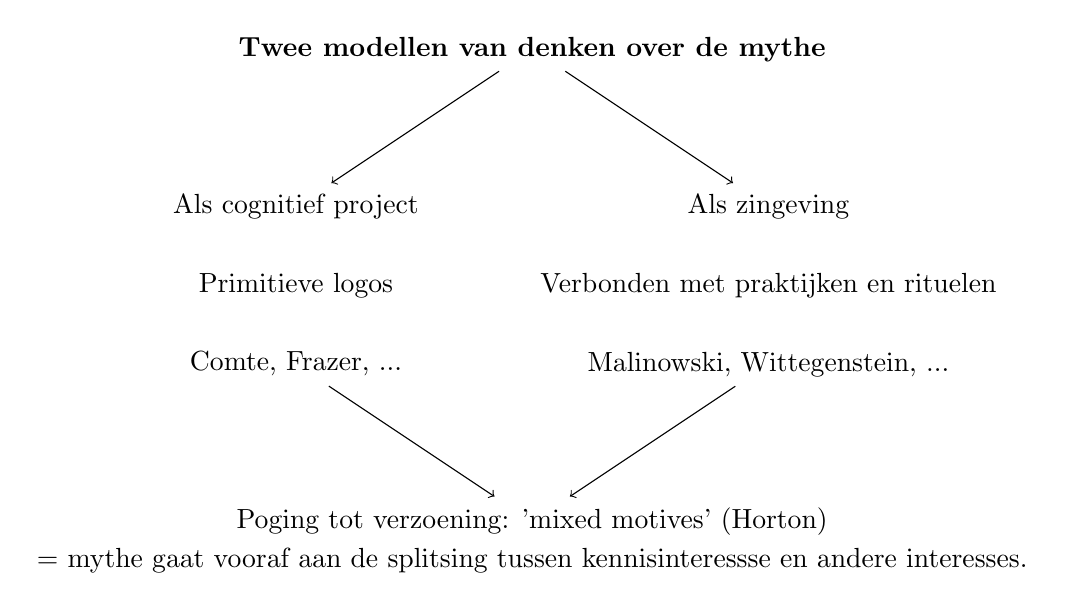
\begin{tikzpicture}[shorten >=1pt,node distance=2cm,on grid,auto] 
\node (a) at (3,0) {\textbf{Twee modellen van denken over de mythe}};
\node (b) at (0,-2) {Als cognitief project};
\node (c) at (6,-2) {Als zingeving};
\node (d) at (0,-3) {Primitieve logos};
\node (e) at (6,-3) {Verbonden met praktijken en rituelen};
\node (f) at (0,-4) {Comte, Frazer, ...};
\node (g) at (6,-4) {Malinowski, Wittegenstein, ...};
\node (q) at (3,-6) {Poging tot verzoening: 'mixed motives' (Horton)};
\node (z) at (3,-6.5) {= mythe gaat vooraf aan de splitsing tussen kennisinteressse en andere interesses.};

\path

(f) edge[->] (q)
(a) edge[->] (b)
(a) edge[->] (c)
(g) edge[->] (q);
\end{tikzpicture}
\end{center}
\section*{\centering \underline{Deel 2: De oude alliantie}}
\section{Alles is water}

\subsection{Inleiding}
\begin{itemize}
\item intrinsiek: van binnen afkomstig
\end{itemize}
\subsection{De ontworsteling van de logos uit de mythos}
\subsubsection{Logos en mythos}
\begin{itemize}
\item presocratici: voor Socrates
\item gonie: oorsprongsverhaal
\end{itemize}
PLATO: Filosofie is geboren uit verwondering.
\\
Mythe is hybride geheel van diverse interesses (cognitief en controle)
\subsubsection{Filosofie/wetenschap}
Filosofie en wetenschap waren \"e\"en, zeker in het oude Griekenland en nog veel later.
\\
WEBER: ontmythologisering van de wereld.
\subsection{De natuurfilosofen en de leer van de elementen}
Speculatieve theorie\"en kwamen tot stand in stadstaten aan de kusten van de Middellandse Zee.
\\
Physis of wordingsbeginsel.
\\Overgaan van krachten/machten naar principes.
De filosofen van toen:
\begin{itemize}
\item Thales van Milete: de "eerste filosoof".
\item Anaximander
\item Anaximenes
\item Herakleitos
\item Parmenides
\item Zeno
\item Democritos: atomisme (=alle stoffen zijn opgebouwd uit ontelbare minuscule ondeelbare blokjes: atomen)
\item Empedocles: grondlegger van de leer van de vier elementen.
\end{itemize}
Ze zoeken naar een minimaal aantal principes (liefst \'e\'en) in de natuur.
\\
\\
Griekse filosofie geobsedeerd door 2 problemen in de natuur:
\begin{itemize}
\item Eenheid en veelheid
\item Verandering en onveranderlijkheid
\end{itemize}
Op zoek naar orde in de chaos.
\\
\\
Elementaire substanties of elementen, die verborgen substantie is achter alle stoffelijke lichamen:
\begin{enumerate}
\item Alles is water: Thales
\item Alles is aarde:
\item Alles is vuur: Pythagoras \& Herakleitos
\item Alles is lucht: Anaximenes
\item (ether)
\end{enumerate}
Deels logos en deels mythos, er zijn \underline{3 ambigu\"iteiten}:
\begin{enumerate}
\item De redenering is: fysisch $\leftrightarrow$ metafysisch
\\-  De elementen zijn fysisch maar de redering is metafysisch.
\\- zie p78.
\item De redenering is: empirisch en concreet $\leftrightarrow$ abstract
\\- zie p78.
\item De redenering is: ratio gebaseerd $\leftrightarrow$ verbeelding
\\- Bachelard: de vier elementen zijn beelden
\\- zie p79.
\end{enumerate}
Gelijkenissen met mythisch denken:
\begin{itemize}
\item Elementen buiten proporties opgeblazen (speculatief, metafysisch en fysich)
\item Oermachten
\item Verbeelding
\end{itemize}
Verschillen met het mytisch denken:
\begin{itemize}
\item Ervaring, empirischme
\end{itemize}
\section{Alles is getal}
Verborgen kennis van de natuur der dingen ligt niet in de waarneming, maar in het wiskundige inzicht: inzicht in wat juist niet waarneembaar is.
\\
Voorbij de ervaring, achter de ervaring zoeken.
\subsection{Opkomst van de wiskundige opvatting van wetenschap}
Vanaf Pythagoras (560-490). De school van Pythagoras had nog wel steeds mystiek trekje.
\\
Mathematisch rationalisme of mathematisch intelectualisme. Met pythagorisme van groot belang als oorsprong van een grote intellectuele traditie in de wetenschap.
\subsubsection{De ontdekking van wiskundige patronen in de natuur}
\begin{itemize}
\item Orfisme: religieuze beweging en leer in de oudheid.
\item Esotherisch: op de grens met de spirualiteit.
\end{itemize}
\subsubsection{De zuivere wiskunde}
\begin{itemize}
\item Incentive: motivatie door het eerst verkrijgeven van een beloning.
\item Ontologie: religieuze beweging en leer in de oudheid.
\end{itemize}
\subsection{De eerste grondslagencrisis}
Werd veroorzaakt door volgende twee aspecten:
\subsubsection{Crisis van de incommensurabele (=onderling onmeetbare) grootheden}
\begin{itemize}
\item Hypotenusa: schuine zijde van een driehoek.
\end{itemize}
EUDOXUS: tijdgenoot Plato, proportie leer $\rightarrow$ was een hulpmiddel om de rekenkunde toch te kunnen gebruiken in de studie van de ruimte.

\subsubsection{De paradoxen van Zeno}
ZENO van Elea, 5e eeuw v.C.,
\section{Alles is idee}

\subsection{De culturele context}
SOKRATES: kennis is in feite ijdelheid en illusie, eeuwige vragensteller.
\subsection{Platoonse idee\"en}
\textit{"De zuivere idee of vorm is de echte structuur van de werkelijkheid, echter dan het waarneembare en ware grondslag van het waarneembare."}
\\
PYTHAGORAS en PLATO: denken dat we middenin de ervaringsmachine zitten.
\\
Waaktoestand tussen droom en realiteit $\rightarrow$ leer van \underline{vier} kennisgraden:
\begin{enumerate}
\item \underline{De kennis van horen zeggen (overlevering, gerucht):} bvb. mytische verhalen.
\item \underline{De informatie van de zintuigen:} min of meer betrouwbare opnie. Betrouwbaar? Mythe van de grot.
Zintuigen leveren niet louter schijn. 
\\ Plato: geen boeddhist $\rightarrow$ zintuigelijke wereld moet participeren aan het echte.
\\
\\
$\longrightarrow$ \textbf{deze twee vormen samen de \underline{doxa}, de opinie}
\item \underline{De kennis door hypothesen:} gefundamenteerde opinie (dianoia) bvb. de mathematiseerbare kennis van de natuur zoals onderandere: acustica, astronomie, statica, hydrostatica, optica...
\\
Echte kennis hoewel hypothetisch.

\item \underline{De kennis vanuit de ware idee (episteme, gezekerde en gefundeerde kennis):}
gerealiseerd door de filosofie, bvb. de reflectie van de axioma's in de wiskunde. Anders moet je tot in het oneindige blijven bewijzen.
\\
Worden aangetoond door reflectie op betekenis van de begrippen (idee\"en) die erin verbonden worden.
\\
\\
$\longrightarrow$ \textbf{deze twee vormen samen de kennis}
\end{enumerate}
De idee van iets is zijn essentie (wezen, eidos) $\rightarrow$ idee\"enleer; de argumenten hiervoor van Plato:
\begin{enumerate}
\item \underline{Het argument van gelijkenissen:} wat we zien belichaamd nooit de hele wezenheid, we spreken telkens over gelijkenissen.
\\
(Een kat een kat noemen)
\item \underline{Het argument van extensie en intensie (denotatie en connotatie):} katten zijn materialisaties van het kattenwezen dat onverandelijk is. De denotatie is niet genoeg om over vaste betekenissen te beschikken.
\item \underline{Type en token:} er moet onderscheid zijn tussen het algemene begrip en het concrete ding. Tokens zijn niet betekenisvol, betekenis vereist abstracties.
\item \underline{Objectiviteit:} wat objectief is leidt een bestaan dat onafhankelijk is van mijn gedachten erover. De kennis van de essentie is ontdekking.
\\
Plato: kennis is de ontdekking van wat er al was.
\end{enumerate}
\subsection{Mathesis en ethiek}
\begin{itemize}
\item \underline{Het $(4+1)$de argument:}
wiskunde heeft de centrale plaats in de kennis.
Door middel van de wiskunde dat we de idee van die gewone dingen, en van minder gewone dingen, kunnen leren kennen.
Wiskundige ideeën leveren in verhouding tot die dingen de modellen: de kennis van de structuur is de kennis van het model van het ding, het modelding.  Model (=idealisering met alleen de essentiële eigenschappen)
\end{itemize}
Ethiek: moddellen voor het menselijk handelen.
\subsubsection*{Dualisme van Plato}
4 grote onderverdelingen westerse filosofie:
\begin{enumerate}
\item Epistemologie: kennisleer, probeert antwoord te geven op vragen als: wat kunnen we kennen en hoe? Zijn er soorten kennis? \dots
\item Metafysica: de ultieme aard van de werkelijkheid, wat bestaat allemaal echt?
\item Antropologie: wil metafysica doortrekken voor de mens en zeggen wat mens in wezen is.
\item Ethiek: wil antwoord geven op de vraag wat het goede leven van die $\uparrow$ mens is.
\end{enumerate}
Plato stelt twee dingen radicaal als tegengestelden tegenover elkaar bvb. lichaam en ziel.
\\
\\
\begin{tabular}{p{4cm} c c p{5cm}}
	\hline
	\hline
	epistemologie & metafysica & antroplogie & ethiek \\
	\hline
	\hline
	zintuigelijke waarneming (doxa) & materie & lichaam, zintuigen & onredelijkheid \\
	\hline
	intellectuele kennis (dianoia en episteme) & Idee, geest & ziel & handelen als participatie aan Idee van het goede \\
	\hline
	\hline
\end{tabular}
\subsection{De mathematische fysica}
PLATO: 
Fysica tussen derde en vierde kengraad. 
De Demiurg.
\\
Vijf elementen, het vijde is het etherische element van de bovenmaanse hemelsfeer.
\\
Alles wordt gespiritualiseerd.
\subsection{Kanttekeningen}
\begin{enumerate}
\item Mytische moteiven, de lee van Plato is een heilsleer die ons wil oproepen ons af te wenden van de illusie en ons te richten naar het echte zijn.
\item Heilsleer van de ratio heeft dubbel karakter: ethische is hoger dan het wetenschappelijk kenbare $\leftrightarrow$ goede ligt in het verlengde van de kennis.
\item Wat ik ken en inzie dat vind ik zelf niet uit.
\item Plato heeft in type en token geen oog voor situaties waar de gehele betekenis staat of valt niet met het algemene, maar juist met het singuliere concrete.
\end{enumerate}
\section{Alles is leven}
\subsection{Van idee\"en naar essenti\"ele eigenschappen}
Model opvatten als abstract begrip in onze geest? Een soort van mentale connotatie (LANGER)?
\\
\\
PLATO: de objectiviteit van het model vereist dat we het begrip ook opvatten als een Idee met een zelfstandig bestaan buiten ons.
\\
\\
ARISTOTELES: was over het algemeen akkoord met Plato maar NIET met de conclusie van hierboven.
\\
\\
"Als kennis van het object kennis is van de essentie van het object, wil dat daarom zeggen dat die essentie zelf een ideaal objecht op zichzelf is?"
\\
\\
Vandaar de argumenten tegen Plato:
\begin{enumerate}
\item De derde man
\item Materie en vorm: de essentie is de vorm voor zover die in de samenstelling met de materie voorkomt.
\item Eigenschappen zijn geen substanties: eigenschappen bestaan in iets anders. Universalia in re.
\item Substantie heeft een essentie. De essentie is niets meer dan een verzameling essenti\"ele eigenschappen die het ding (naast toevallige eigenschappen) bezit.
\end{enumerate}


\subsection{Biologie, fysica en (een beetje) metafysica}
ARI: Wiskunde heeft niet de centrale plaats in de kennis. 
\\
\\
Graden van abstractie:
\begin{itemize}
\item De fysiche abstractie: mengelvorm van empirisch en ratioeel denken die past bij natuurobjecten (levende dingen).
\item De wiskundige abstractie: past bij wiskundige objecten en natuurobjecten die een wiskundige regelmaat vertonen zoals het "bovenmaanse"; bvb. de astronomie.
\item De metafyische abstractie: datgene dat alle objecten aan kenmerken moeten bezitten om \"uberhaupt te bestaan.

\end{itemize}

De natuurwetenschapen splitsen zich in twee:
\begin{enumerate}
\item Wiskundige disciplines: bovenmaanse natuur.
\item Levenswetenschappen en ervaringswetenschappen: ondermaanse natuur.
\end{enumerate}
$\rightarrow$ de band tussen wiskundige en ervargingswetenschappen gaat voor vele eeuwen verloren.
\subsection{Logica}
Syllogisme: de eerste echte logische theorie door Ari.
\subsection{Moraal en praktische filosofie}
Doel en moraal van het leven zijn dezelfde: vorm van welslagen vinden dat de gelukkige mens kenmerkt. Gelukkige leven (eudaimonia) is een kwestie van deugd.
\\
\\
Phronesis de meest typische aristotelische deugd: redelijke inzicht in de aard der dingen dat in staat is ook evenwicht te bereiken in het handelen in overeenstemming met die aard der dingen.
\subsection{Kanttekeningen}
'Trouble with Ari': door zijn empirisch realisme bereik van wiskunde fel ingeperkt.
\section{Alles is bedoeld}
\subsection{De kentering}
Na Plato en Ari: theoretische filosofie over zijn hoogtepunt heen.
\\
Romeinen vonden niets nieuw uit in de filosofie en gebruikten enkel de wiskunde van de Grieken. 
\\
Wel vonden ze de technische interesse opnieuw uit.
\subsection{Bilan van het antieke denken. De derde factor}
\subsubsection{Twee concepties}
\begin{enumerate}
\item Filosofie als uiting van zuiverste kennisdrang.
\item Filosofie gericht op 'levenswijsheid".
\end{enumerate}
\subsubsection{De derde factor}
\begin{enumerate}
\item[3.]Zin-interesse.
\end{enumerate}
Ontstaan alliantie tussen de kennisinteresse en de ‘derde factor’.
\subsubsection{Twee stromingen}
De eerste conceptie in paragraaf \"e\"en moet nog onderverdeeld worden in:
\begin{enumerate}
\item Epirische onderzoekstraditie.
\item Rationalistische onderzoekstraditie.
\end{enumerate}
\subsection{De christelijke middeleeuwen}
Niet tegen de rede, maar op zoek naar verzoening ermee.
Filosofische basis: neoplatoonse school: PLOTINUS, PROCLUS (300 n.C.) Eerste synthese AUGUSTINUS.
ARI in de arabische cultuur. Dus naast wiskundige wetenschappen (begrijpbaar voor Christenen) ook: biomed. ervaringswetenschappen, anatomie, biologie, fysica en geneeskunde.
Westen onder de indruk, vertaalcampagne: ARI, grote Arabische denkers (AVICENNA en AVERROES).
1250: eerste universiteiten strijd: platonisten vs. Averroïsten.
-> Synthese door Thomas van AQUINO
\\
\\
God heeft de natuurlijke wereld zo willen scheppen dat hij voor mensen met hun natuurlijke rede kenbaar is.
\\
\\
APOTHEOSE van de ALLIANTIE tussen KENNIS en ZINGEVING.
\subsection{Doeloorzakelijkheid}
Goddelijk scheppingsplan biedt natuurlijk inspiratiekader voor de doeloorzakelijkheid waar ARI op hamerde. (De schepping is duidelijk bedoeld.)
\\
4 oorzaken volgen Ari:
\begin{enumerate}
\item Materi\"ele oorzaak: materiaal om iets te bouwen.
\item Effici\"ente oorzaak: handeling van de maker.
\item Formele oorzaak: de vormen of essenties die de materie kan aannemen.
\item Dooloorzaak: de bestemming van het eindproduct.
\end{enumerate}
Finalistisch of teleologische denkwijze: er steeds voor alles een doeloorzaak, een telos of doel waarnaar het natuurzijnde streeft.
\section*{\centering \underline{Deel 3: De nieuwe alliantie}}
\section{Experimenteel empirisme}
\subsection{Een harmonische keurslijf?}
De oude alliantie: kennis en zingeving zijn een tweespan.
\\
V.a. 1300-1400 dus jonge universiteiten met dominante aristotelische traditie en een scheutje platonisme erin.
\\
2 eeuwen later (herfsttij van de middeleeuwen) aristotelisch denken ondergraven door 2 tendensen: nieuw radicaal empirisme en heropleving platonisme.
\\
Desintegratie middeleeuwse synthese.
\subsection{Gemeenschappelijke punten van kritiek}
Nieuwe empiristen en platonisten kritiek tegen scholastisch denken.
\\
\\
TURGOT: “Zolang zij nog niet echt verlicht waren over de natuurlijke toedracht der dingen, stelden de filosofen zich voor dat zij de oorzaken van de verschijnselen verklaarden door middel van algemene uitdrukkingen zoals essentie of kwaliteit, woorden die nochtans niets verklaren.”
\\
\\
De empiristen en platoons kwamen overeen voor de volgende punten van kritiek:
\begin{enumerate}
\item Fameuze doeloorzaken verklaren niks (zeggen dat de neus doelmatig gemaakt is zodat de bril er op past).
\item Parodie op syllogisme. (Enkel reeds bekende gegevens op een rijtje zetten)
ECO en RABELAIS.
\\
Welke is de ware methode? Inductieve of mathemathische methode.
\item Beperking: wetenschap zou gewoon een verlengstuk zijn van het ‘gezond verstand’. \textit{Common sense} is een t\'e smalle basis:
\\We nemen steeds alleen waar wat we begrippelijk kunnen vatten en plaatsen: iemand die nooit van elktronen heeft gehoord zal geen elktronenspoor zien, ook niet wanneer men hem de juiste waarnemingsinstrument geeft.
\end{enumerate}
\subsection{Empiristische kritiek en alternatief}
Kritiek van de empiristen:
\begin{enumerate}
\item Te veel laten leiden door vooropgezette ideeën en vertrouwde begrippen. De waarneming moet gezuiverd worden van a priori's die haar besmetten.
\\Het komt er op aan, te komen tot zuivere waarneming zonder theorie.
\item Theorie moet achteraf worden opgebouwd op basis van inductie.
NIET de DEDUCTIE van het syllogisme maar de INDUCTIE uit de feiten.
\\
BACON,OCKHAM en GROSSETESTE
\item Radicale taalfilosofie: nominalisme. Echte inhoud ligt in de empirische invulling. 
\\
G\'e\'en universalia meer (wel nog bij platonisten en aristotelici)
Nominalisme met 2 gezichten: polemisch (toen heersende wetenschap ontmaskeren) en ‘algemene labels’ nu eenmaal nodig (iets anders dan wat de ervaring je zelf opdringt)
\\
GOODMAN, HACKING en FOUCAULT
\end{enumerate}
\begin{quote}
Allemaal redelijk naief:
\begin{enumerate}
\item[1*] Waarneming verstonderstelt altijd interpretatie en dat gebeurt altijd vanuit een theorie).
\\
“En net zoals de blinde zal de zuivere waarnemer niets zien – tenzij chaos, zoals PLATO al opmerkte”
\item[2*] Als er geen zuivere waarneming voorafgaat aan de hypothese, waar beginnen om zuiver inductief te werk te kunnen gaan?
\item[3*] Tot op vandaag onenigheid over nominalisme. Kunnen we anders dan met algemene begrippen de empirie te lijf gaan?
\end{enumerate}
\end{quote}
\begin{enumerate}
 \item[4.] Experiment als revolutionair idee. Actieve ervaring is meer dan louter kijken, meer dan zelfs kijken door de bril van hypothesen.
\end{enumerate}
\begin{flushleft}
\begin{tabular}{p{6cm} p{5cm} p{4cm}}
	\hline
	
	 \raggedright Aristotelisch essentialisme (scholastiek) & Bacons alternatief (experimenteel empirisme) & Vraagtekens bij het alternatief\\
	\hline
	\begin{flushleft}
	\begin{enumerate}
	
	\item \textit{commons sense} interpretatie van de waarneming (metafysich, met doeloorzaken)
	\item abstract \textbf{deductieve} methode (syllogisme)
	\item essenties en universalia
	\item passieve waarneming, representatie van de natuur
	\end{enumerate}	 
	\end{flushleft}
	
	&
	\begin{flushleft}
	\begin{enumerate}
	\item \textbf{pure waarneming}, zuivere empirie, brute feiten
	\item \textbf{inductie} (veralgeming van feiten tot wetten)
	\item \textbf{nominalisme}
	\item \textbf{experiment,} active waarneming, interventie
	\end{enumerate}
	\end{flushleft}
	&
	
	\begin{flushleft}
	\begin{enumerate}
	
	\item waarneming is ge\"interpreteerd (Gestalten)
	\item hypothetisch- deductieve mehtode
	\item patstelling?
	\item OK!
	
	\end{enumerate}
	\end{flushleft}

	\\
	
	\hline
	
\end{tabular}
\end{flushleft}
\section{Rationalisme}
Niet te kennen!
\section{Spanning en samenspel}

\begin{figure}
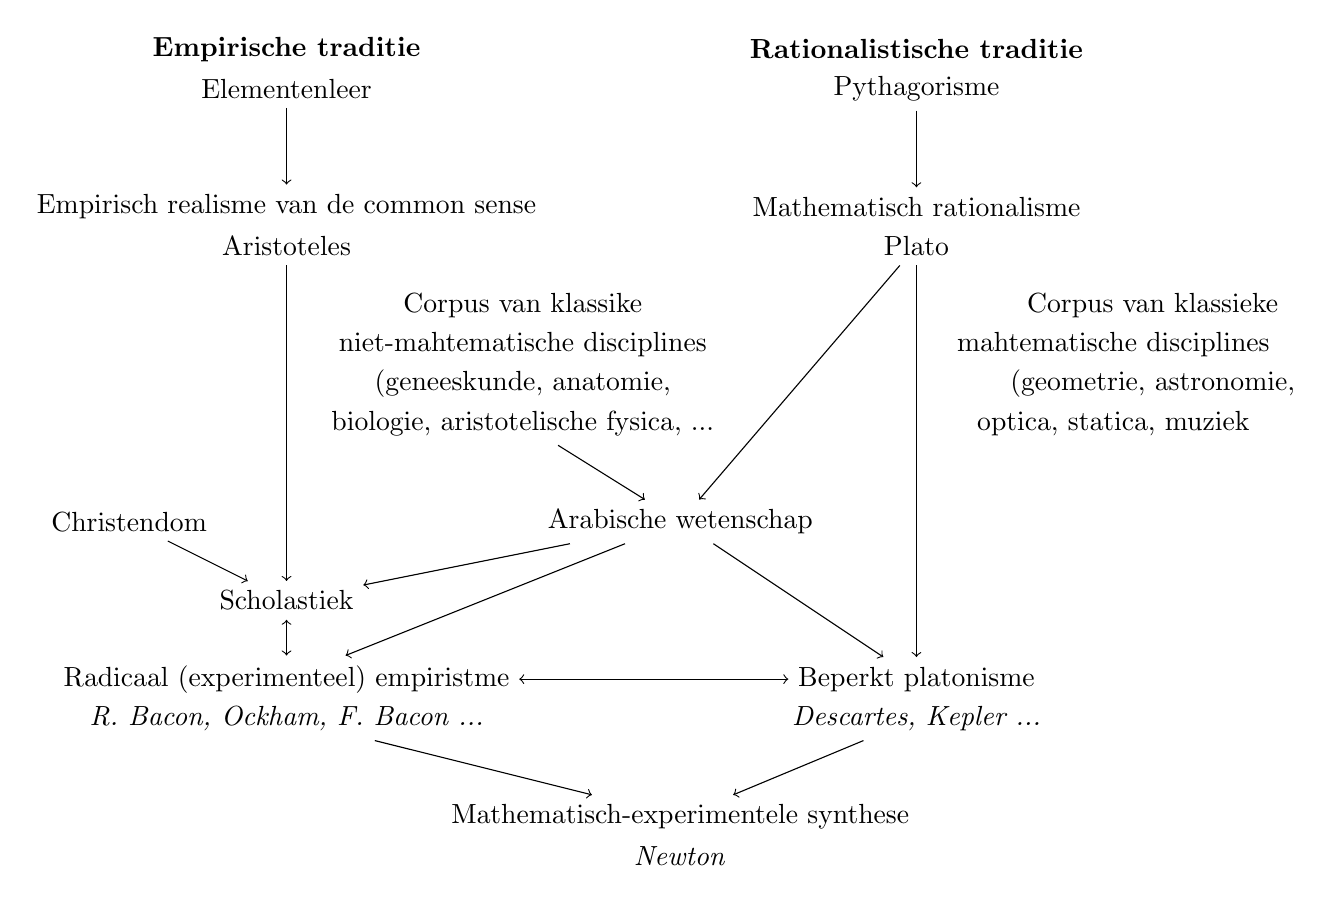
\begin{tikzpicture}
\node (a1) at (-20,0) {\textbf{Empirische traditie}};
\node (a2) at (-12,0) {\textbf{Rationalistische traditie}};
\node (b1) at (-20,-0.5) {Elementenleer};
\node (b2) at (-12,-0.5) {Pythagorisme};
\node (c1) at (-20, -2) {Empirisch realisme van de common sense};
\node (c2) at (-12, -2) {Mathematisch rationalisme};
\node (d1) at (-20,-2.5) {Aristoteles};
\node (d2) at (-12, -2.5) {Plato};

\node (et1) at (-17,-3.25) {Corpus van klassike};
\node (et2) at (-17,-3.75) {niet-mahtematische disciplines};
\node (et3) at (-17,-4.25) {(geneeskunde, anatomie,};
\node (et4) at (-17,-4.75) {biologie, aristotelische fysica, ...};

\node (ft1) at (-9,-3.25) {Corpus van klassieke};
\node (ft2) at (-9.5,-3.75) {mahtematische disciplines};
\node (ft3) at (-9,-4.25) {(geometrie, astronomie,};
\node (ft4) at (-9.5,-4.75) {optica, statica, muziek};

\node (g1) at (-22, -6){Christendom};
\node (g2) at (-15, -6){Arabische wetenschap};

\node (h) at (-20,-7){Scholastiek};
\node (i1) at (-20, -8){Radicaal (experimenteel) empiristme};
\node (i2) at (-12, -8){Beperkt platonisme};

\node (j1) at (-20, -8.5) {\textit{R. Bacon, Ockham, F. Bacon ...}};
\node (j2) at (-12, -8.5) {\textit{Descartes, Kepler ...}};

\node (k) at (-15, -9.75) {Mathematisch-experimentele synthese};
\node (l) at (-15, -10.25) {\textit{Newton}};


\path
(b1) edge[->] (c1)
(b2) edge[->] (c2)
(d1) edge[->] (h)
(d2) edge[->] (i2)
(d2) edge[->] (g2)
(et4) edge[->] (g2)
(g1) edge[->] (h)
(g2) edge[->] (h)
(g2) edge[->] (i1)
(g2) edge[->] (i2)
(h) edge[<->] (i1)
(i2) edge[<->] (i1)
(j1) edge[->] (k)
(j2) edge[->] (k);
\end{tikzpicture}
\end{figure}

\begin{itemize}

\item De enkelvoudige pijlen stellen lijnen van be\"invloeding voor, de dubbele pijlen tegenstellingen (die soms ook verwantschap insluiten).
\item Beide grote lijnen zijn onderweg van buitenaf be\"invloed, door christendom en Arabische wetenschap en filosofie (en de traditie van de magi).
\end{itemize}

\section{Kritiek en constructie}
\subsection{Een dubbelzinnig scepticus?}
HUME neemt de empiristische erfenis van de BACONs over en werkt die uit tot een even indrukwekkende filosofie als die van de rationalisten, maar totaal anders ge\"orienteerd.
\\
Nooit iets meer dan de waarschijnlijkheid kunnen bereiken.
\\
Herhaling en gewoonte  oorzaak en gevolg. Zeker zijn van twijfel. 
\\
HUME wil ons bevrijden van de zoektocht naar onze schijnzekerheden.
\\
\\
Slotsom: Kennis is een bouwsel opgetrokken van op de ervaring, en de beste theorieën die we daaruit induceren zijn waarschijnlijke hypothesen. 
\\
\\
\textbf{Drie putnen van twijfel, drie praktische zekerheden:}

\begin{enumerate}
\item \textbf{Causaliteit:} 
\begin{itemize}
\item Niet meer dan de vaste opeenvolging van fenomeen A en fenomeen B in de waarneming: een gewoont (associate), dus subjectief.
\item Een natural belief.
\end{itemize}

\item \textbf{Inductieprobleem:}
\begin{itemize}
\item Logische sprong; einde van de zekerheid; oplossing: geen radicaal maar gematigd scepticisme; overgang naar waarschijnlijkheid.
\item Een natural belief.
\end{itemize}

\item \textbf{Personal identity}
\begin{itemize}
\item Een constructie, er is alleen een $+/-$ continue bewustzijnstroom
\item Een natural belief: \begin{itemize}
\item Sociaal: we maken elkaar in de omgang tot vaste personen.
\item Criterium van lichamelijke continu\"iteit doorheen tijd en ruimte.
\end{itemize}
\end{itemize}
\end{enumerate}
\subsection{De onverbiddelijke verzoener}
Niet te kennen!
\subsection{Kantiaans constructivisme}
Niet te kennen!
\subsection{... en de zin van alles?}
Niet te kennen!
\section{Positivisten en popperianen}
Niet te kennen!
\section*{\centering \underline{Deel 4: Hoe overleven we de wetenschap?}}
\section{De tafel van Eddington}
\subsection{Het wetenschappelijke en manifeste beeld}
Arthur EDDINGTON (1882-1944): \textit{Stel dat de atoomtheorei klopt, dan zijn tafels en stoelen in feite niets dan een hoop atomen en nog kleinere partikels dwarrelend in een lege ruimte?!}
\\
$\rightarrow$ De ervaring is dan een subjectieve machine, een fabriek van illusies bovenop de echte onderliggende realiteit met haar andere, onzichtbare gezicht.
\\
\\
EDDINGTON zocht oplossing voor dit dilemma:
\\
Aannemen van complementarieit of correspondentie tussen beide beschrijvingsniveaus.
\\
\\
Wilfrid SELLARS (1912-1989): veralgemeent probleem van EDDINGTON $\rightarrow$ het gaat niet alleen over macroscopische objecten, maar de gehele leefwereld.
\\
Twee beelden van de realiteit:
\begin{enumerate}
\item Wetenschappelijke beeld
\item Manifeste beeld
\end{enumerate}
Volgens SELLARS moet je kiezen tussen de twee beelden:
\begin{enumerate}
\item De argumenten pleiten voor een vorm van realisme, ze willen weten het nu echt zit, los van voorstellingen: dan kan met niet evenveel geloof hebben in beid.
\item Beide beelden maken een totaalclaim.
\item Het succes-argument: wetenschap is een \textit{succes story}, het manifeste beeld is dat niet. In alle gebiede buite dat van beweste menselijke ervaring heeft wetenschappelijke beeld gewonne van het manifeste. SELLARS zegt dat de wetenschappen van de mens onderdeel moeten worden van de natuurwetenschappen.
\end{enumerate}
De argumenten roepen veel vragen op, vooral rond de premissen realisme en totaalbeelden:
\begin{enumerate}
\item[i.] Je verwerpt beide premissen:
\newtheorem*{def1}{Pragmatisch pluralisme}
\begin{def1}
Wie bv. meent dat wetenschappelijke theorie\"en de beste instrumenten zijn om aan fysica, chemie en biologie te doen, maar het manifeste common sense beeld (inclusief folk pychology) het beste instrument om aan psychologie, esthetica, ehtica, pedagogiek en didactiek, talen, geschiedenis, dagelijkse communicatie enz. te doen.
\end{def1}

\item[ii.] Je aanvaardt totaalclaims maar verwerpt realisme:
\newtheorem*{def2}{Instrumentalisme}
\begin{def2}
Wie bv. meent dat wetenschap in het algemeen overal het beste instrument is om kennis te hebben (totaalclaim), maar daarom niet als een letterlijk beeld van de realiteit gezien moet worden. Of andersom: dat het manifeste overal het beste instrument levert om de wereld te bespreken, maar daarom nog niet letterlijk waar.
\end{def2}

\item[iii.] Je aanvaardt realisme maar verwerpt totaalclaims:
\newtheorem*{def3}{Realistisch pluralisme}
\begin{def3}
Wie bv. meent dat wetenschap het beste realisitsche beeld is om fysica, biologie, enz. te doen \'en het manifeste common sense beeld (inclusief folk psychology) het beste realisitsche beeld om aan psychologie, esthetica, ethica, didactiek, ... te doen.
\end{def3}

\item[iv.] Beide premissen aanvaarden maar die van bv. realisme beperkter:
\newtheorem*{def4}{Compatibilisme I}
\begin{def4}
Wie bv. meent dat wetenschap het beste realistische beeld geeft van alles, en common sense het beste instrument om minstens een deel van de fenomenen te bespreken (bv. in de psychologie, enz.).
\end{def4}
\item[v.] Beide premissen aanvaarden maar die van bv. realisme beperkter:
\newtheorem*{def5}{Compatibilisme II}
\begin{def5}
Wie bv. zegt: wetenschappelijke psychologie is wellicht het beste beeld, realistisch of misschien zelfs ook los van realisme, als het op de objectieve (zo objectief mogelijke) kennis aankomt van de geest; maar common sense is het beste, zelfs het enige beeld dat ons toelaat andere da zuiver cognitieve taal te spreken over de geest enz. Zo bv. om over de zin (of onzin!) van dingen te spreken, om over mensen, menselijke communicatie en verhoudingen te spreken, om over cultuur te spreken: we kunnen bv. niet over mensen als mensen (dus als \'e\'er dan machines) spreken zonder ze als personen te beschouwen, en we kunnen dan weer niet over personen spreken zonder ze beliefs \& desires toe te schrijven.
\end{def5}
\end{enumerate}

\textbf{Overzicht: mogelijke alternatieven voor SELLARS}
\\
\begin{tabular}{l c c}
\hline
realisme totaalbeeld & - & +
\\
- & pragmatisch pluralisme (i) & instrumentalisme (ii)
\\
+ & realistisch pluralisme (iii) & compat. I (iv) compat. II (v)
\\
\hline
\end{tabular}
\subsection{Metafysisch realisme en science freaks}
De idee dat je over de wereld ook voor zover die zich gedeeltelijk aan de waarneming onttrekt een beeld, een theorie moet opstellen, die je op zijn beurt voor waar of onwaar moet houden.
\\
Volgens deze vorm van wetenschappelijk realisme wordt wetenschap de 'echte metafysica':
\begin{enumerate}
\item Realisten: er bestaat objectieve kennis over alles.
\\
Antirealisten: er bestaan enkel objectieve kennis voer waarneembare realiteit.
\item Het samenspel van ratio en experimentele empirie geeft betekenis aan elke objectiviteit.
\item Samenspel van kennis en controle. Wetenschap de absolute conception of reality, opgesteld van een volledig extern standpunt. Als dit zo is, dan is verandering en beheersing geen onderdeel van haar project. Elke menselijke interesse is er vreemd aan. Wetenschapper wordt goddelijk, ziet alles vanuit pure theoria
\\
\\
$\Rightarrow$ Hoe overleven we zo'n wetenschap?
\end{enumerate}
\section{De bessen van mijn jeugd}
\subsection{Twee echtheden, drie graden van belichaming}
LANGER: opvatting volgens dewelke we alleen door instrumentele interesses worden gedreven, moeilijk in overeenstemming is te brengen met onze gerichtheid op symbolen.
Iets méér dan een interesse om te weten. (Symbolische erkenning bij voorbeeld met de biologische vader)
Het ‘echte kennen’ is weten hoe het is, los van het verlangen dat het zus of zo zou zijn.
\\
\\
Fundamentele interesses, symoblisch op twee gronden:
\begin{enumerate}
\item Menselijk symbolisch systeem van taal.
\item Gebruik van symbolen in een tegelijk striktere en bredere, maar alleszins pertinente zin. Symbolen hebben een intrinsiek belang.
\end{enumerate} 

Toegepast op de fundamentele interesses:
\begin{enumerate}
\item Kennis wetenschap) als techniek (controle, beheersing) en zingeving zijn symbolisch: zij hebben de taal nodig om gecommuniceerd en van generatie op generatie doorgegeven te worden.
\item Verschil tussen de drie interesses:
\begin{itemize}
\item Zwak belichaamde betekenissen: techniek maakt weinig of geen gebruik van strikte symbolen. 
	Wetenschap: méér sprake van intrinsieke symbolen.
\item Matig belichaamde betekenissen: kennisinteresse is in de eerste plaats intrinsiek (weten uit een drang om te weten) LAPLACE, PRIGOGINE
De betekenis van wetenschappelijke stellingen kun je in verschillende graden van exactheid en moeilijkheid omschrijven of benaderen. 
\item Sterk belichaamde symbolen: derde interesse (zingeving), niet mogelijk afstand te doen van de symbolen. 
\end{itemize}
\end{enumerate}
De betekenis van sterk belichaamde symbolen is evocatief en ondoorzichtig, die van informatieve taal expliciet en transparant. 
\subsection{De drie interesses: contaminatie en behoud van verschil}
Moderne wetenschap $\rightarrow$ alliantie met de techniek. De vraag naar de zin naar een aparte sfeer verwezen. 
\\
De rationaliteit en haar grenzen. BURMS en DE DIJN
\\
Wetenschap is een empirische praktijk die in het verlengde ligt van de common sense. Geen re\"ele bedreigingen kunnen uitgaan van de ene interesse voor de andere. Interesses kunnen elkaar wel in het gedrang brengen door een soor van verwarring in de hoofden van de mensen. 
Ook de mythe is een kluwen geweest van interesses. HORTON
Co-existentie.
\subsection{... en het magisch symbolisme?}
Waarom geïnteresseerd zijn in iets dat evengoed gesimuleerd kan worden?
\\
Geen empirisch verschil, dan kan de fascinatie (en ontgoocheling) enkel een kwestie zijn van ‘magie’. Verschil zit in de eigen symbolische houding. 
\\
STENDHAL, ALAIN-FOURNIERS en LEVI
\end{document}